\documentclass[12pt,titlepage]{article}
\usepackage[left=2cm,top=2cm,bottom=2cm,right=2cm]{geometry}
\geometry{a4paper}
\usepackage[parfill]{parskip}
\usepackage{auto-pst-pdf}
\usepackage{graphicx}
%german compatibility
\usepackage[ngerman]{babel}
	\selectlanguage{ngerman}
\usepackage[utf8]{inputenc}
\usepackage[T1]{fontenc} 

\usepackage{mathabx} % for math symbols
\usepackage{pstricks}
\usepackage{pst-circ}
\usepackage{gnuplottex}
	\usepackage{latexsym}
	\usepackage{keyval}
	\usepackage{ifthen} 
\usepackage{rotating}
%\usepackage{SIunits}
%\usepackage{listings} % for code listings
\usepackage{listingsutf8}
\lstset{
    extendedchars=\true,
    inputencoding=utf8/latin1,
    breaklines=true,
    numbers=left,
    escapeinside={<!}{?>}
}
\usepackage{struktex}
%\usepackage{german} % used by struktex
%\usepackage{fontspec,xltxtra,xunicode}
\usepackage{pmboxdraw} %used for building oscillator symbol
\usepackage[compact]{titlesec}
\usepackage{mdwlist} %for compact lists and so on...

%pdf mods
\usepackage{booktabs} % for much better looking tables
\usepackage{array} % for better arrays (eg matrices) in maths
\usepackage{paralist} % very flexible & customisable lists (eg. enumerate/itemize, etc.)
\usepackage{verbatim} % adds environment for commenting out blocks of text & for better verbatim
\usepackage{subfig} % make it possible to include more than one captioned figure/table in a single float
% These packages are all incorporated in the memoir class to one degree or another...
\usepackage[bookmarks=false,linkcolor=blue,pdfstartview={XYZ null null 1.22},unicode]{hyperref}
\hypersetup{pdfborder= 0 0 0}

\title{\vspace{-1.5cm}Raumklimaerfassung mit Monoflop und Thermistor\vspace{-5mm}}
\author{Gruppenmitglieder: \input{names.txt}\\
			  Autoren: \input{authors.txt}}
\date{\vspace{-2mm}\today}

\begin{document}
	%\thispagestyle{empty}
	\maketitle
	\tableofcontents	
	\newpage
	
	\section{Schaltung}
		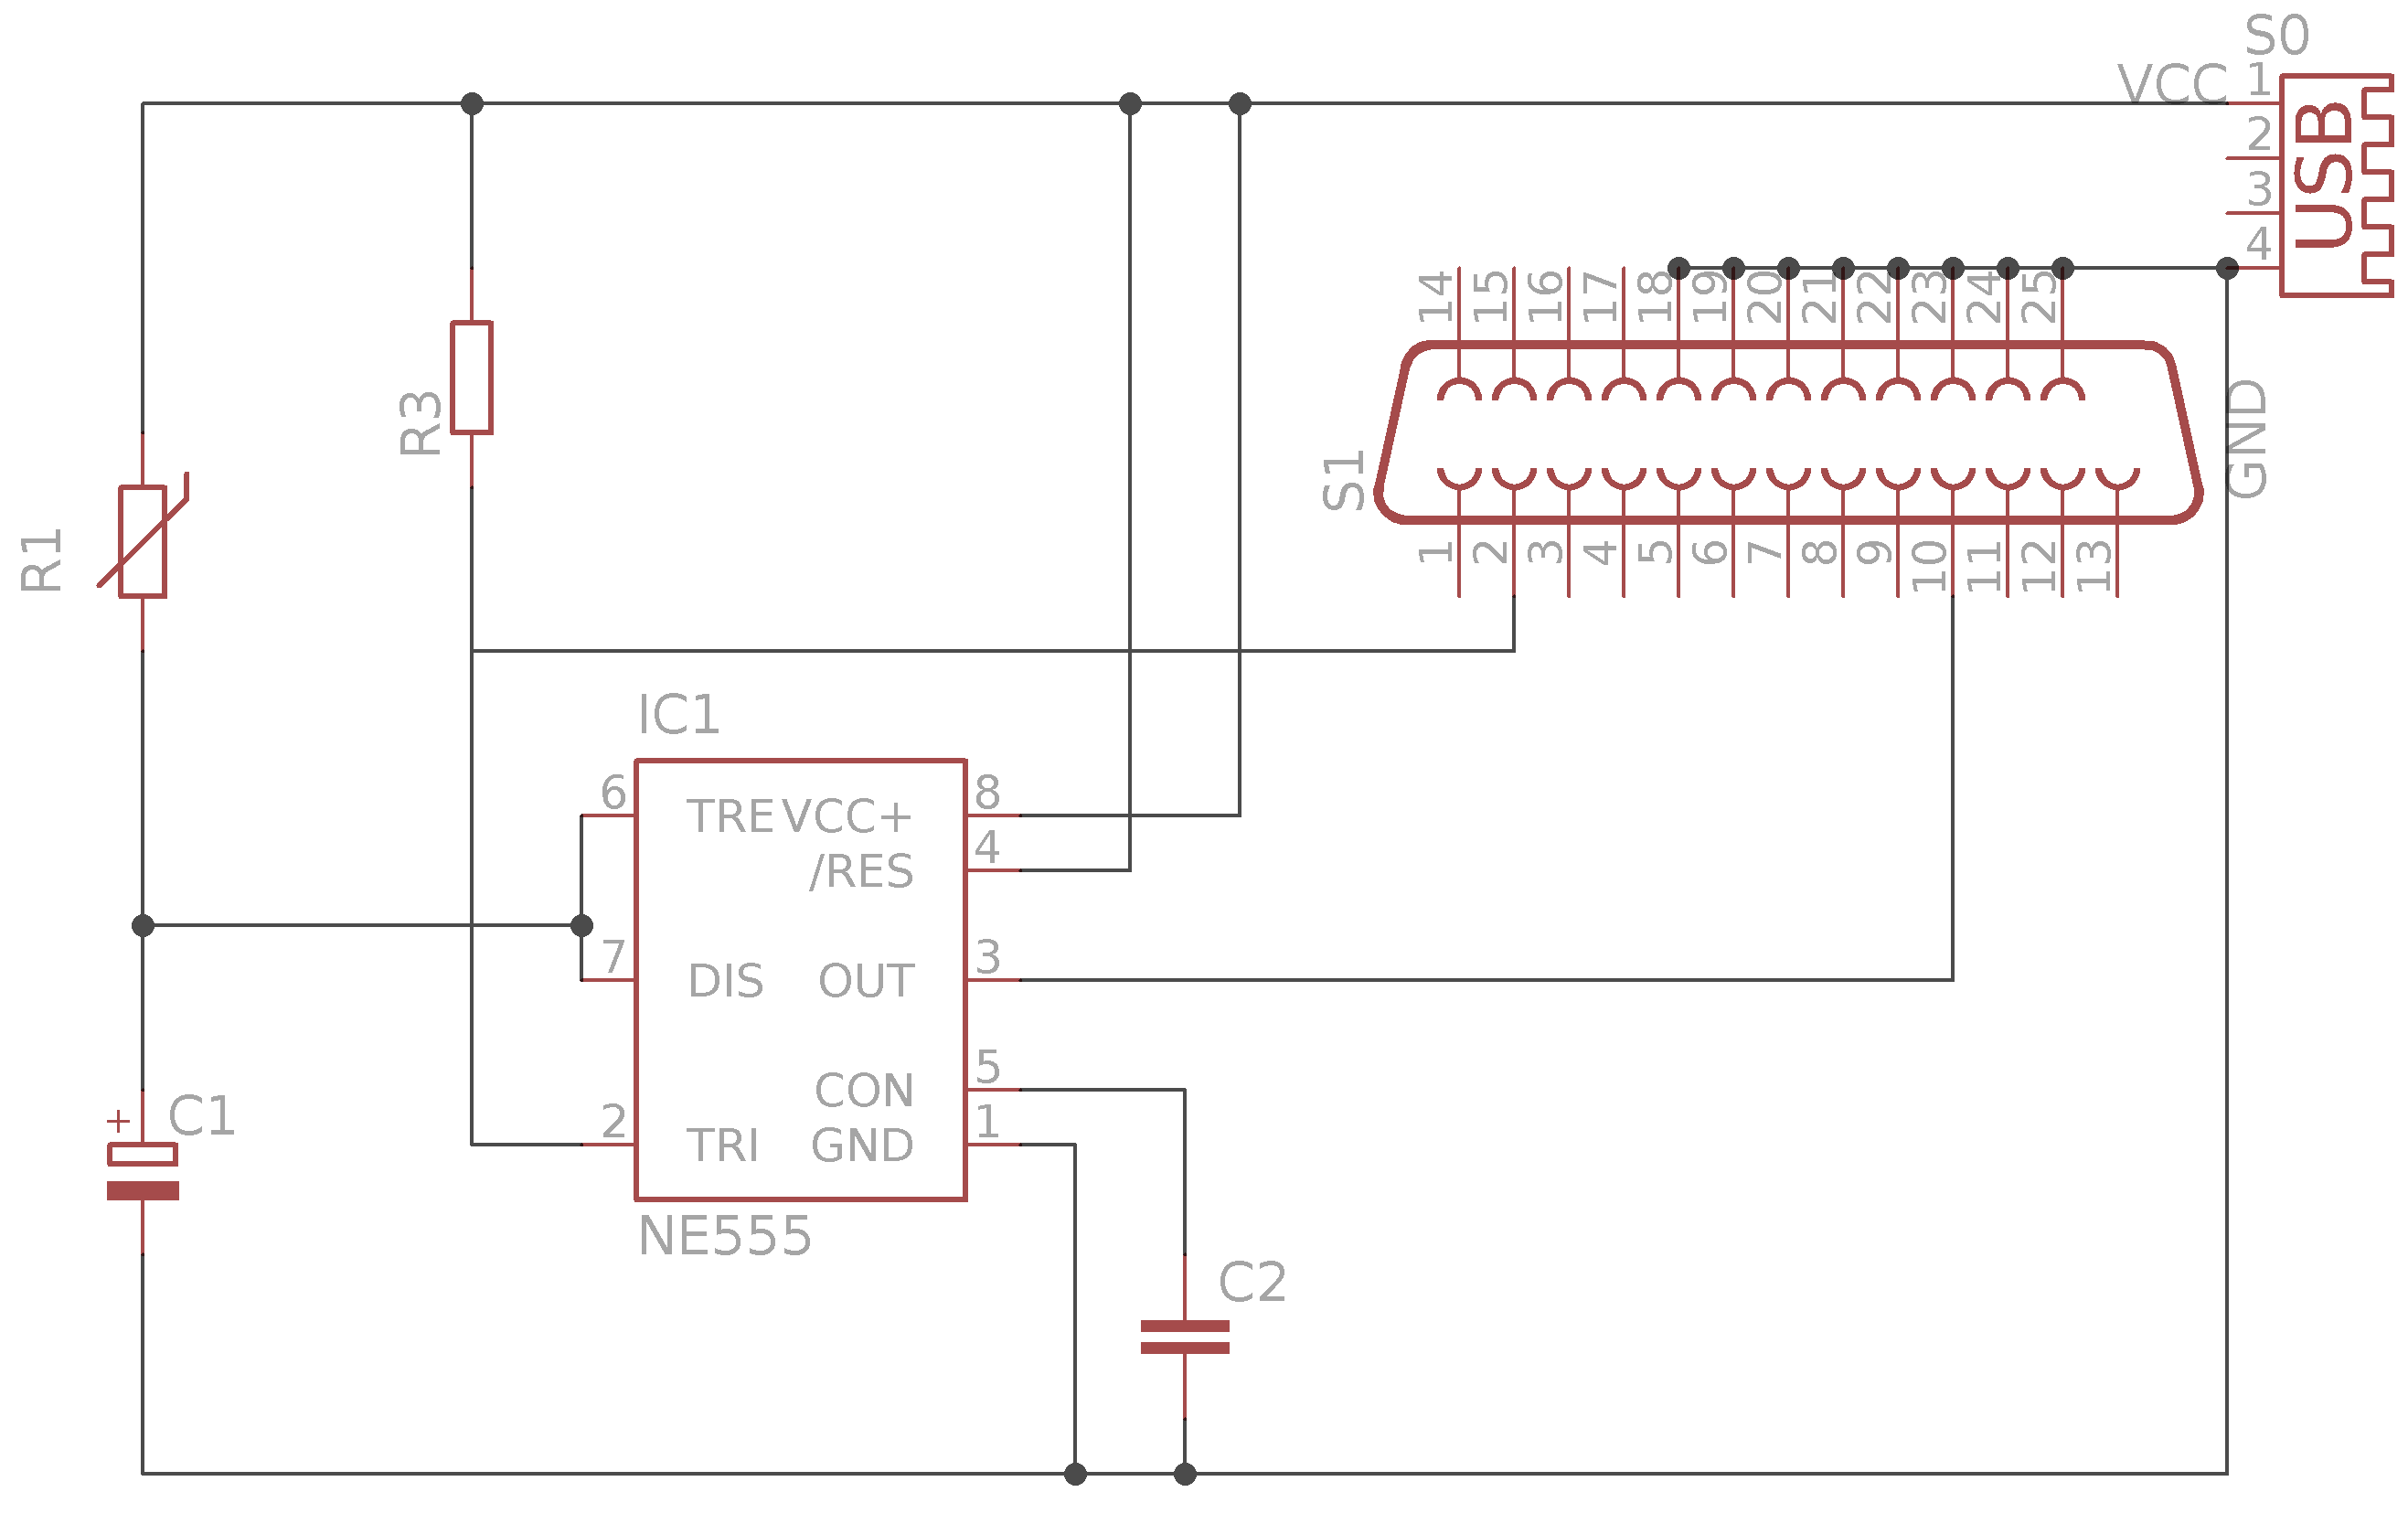
\includegraphics[scale=1.5]{res/Schematik.png}
%	\begin{pspicture}[showgrid=false](12,5)
%		\pnode(0.75,5){A}
%		\pnode(0.75,0){B}
%		\Ucc[labeloffset=0.85](A)(B){$V_{cc}$}
%		\pnode(2,5){C}
%		\wire(A)(C)
%		\pnode(2,1.5){D}
%		\wire(C)(D)
%		\pnode(3,1.5){P4} % pin4
%		\wire(D)(P4)
%		\pnode(2.5,0){E}
%		\wire(B)(E)
%		\pnode(2.5,3){F}
%		\pnode(3,3){P1} %pin1
%		\wire(E)(F)
%		\wire(F)(P1)
%		\pnode(3,5){G}
%		\wire(C)(G)
%		\pnode(3,2.5){P2} % pin2
%		\resistor[labeloffset=-0.6](G)(P2){$R_{2}$}
%				
%		\logicic[nicpins=8,%
%			pinalabel=GND,pinblabel=TRG,pinclabel=OUT,pindlabel=RST,%
%			pinelabel=CVtg,pinflabel=TRS,pinglabel=DCG,pinhlabel=$V_{cc}$,%
%			pinanumber=1,pinbnumber=2,pincnumber=3,pindnumber=4,%
%			pinenumber=5,pinfnumber=6,pingnumber=7,pinhnumber=8,%
%		](3,1){NE555}
%
%	%Connect P8		
%		\pnode(7.5,3){P8}
%		\pnode(7.5,5){O}
%		\wire(P8)(O)
%		\wire(G)(O)
%		
%		% Connect P6
%		\pnode(7.5,2){P6}
%		\pnode(7.5,2.5){P7}
%		\wire(P6)(P7)
%		
%		%connect P7 to middle of VD
%		\pnode(10,2.5){T}
%		\wire(P7)(T)
%				
%		%dirty pinconnector
%		\pnode(11.5,4){PC0}
%		\pnode(12,4){PC1}
%		\pnode(11.5,1){PC3}
%		\pnode(12,1){PC4}
%		\wire(PC0)(PC1) \wire(PC0)(PC3) \wire(PC3)(PC4) \wire(PC4)(PC1)
%		\pnode(11.75, 3.25){D1} % data 1
%		\pnode(11.75, 3){D2} % data 2
%		\pnode(11.75, 1.5){PCGND}
%		\newground(PCGND)	\pscircle *(D1){2\pslinewidth}	\pscircle *(D2){2\pslinewidth}	
%		\rput(14,3){DB-25--Schnittstelle}
%		
%		%Connect D1
%		\pnode(3,0.75){H}
%		\pnode(3,2){P3} % pin3
%		\wire(H)(P3)
%		\pnode(8,0.75){I}
%		\wire(H)(I)
%		\pnode(8,3.25){J}
%		\wire(I)(J)
%		\wire(J)(D1)
%		
%		%Connect D2
%		\pnode(2.75, 2.5){K}
%		\wire(P2)(K)
%		\pnode(2.75,0.5){L}
%		\wire(K)(L)
%		\pnode(8.2,0.5){M}
%		\wire(L)(M)
%		\pnode(8.2,3){N}
%		\wire(M)(N)
%		\wire(N)(D2)
%		
%		%draw voltage divider
%		\pnode(10,5){R}
%		\pnode(10,0){S}
%		\multidipole(R)(S)\resistor[dipolestyle=varistor]{$R_1$}%
%			\wire%[intersect,intersectA=A,intersectB=B]%
%		\capacitor{$C_1$}.
%		\wire(O)(R)
%
%		%connect ground of data port to usb ground
%		\pnode(11,0){P}
%		\wire(E)(P)
%		\pnode(11,1.5){Q}
%		\wire(P)(Q)
%		\wire(Q)(PCGND)
%		
%		%connect P5 w/ anti-noise capacitor to ground
%		\pnode(9.1,1.5){U}
%		\pnode(7.5,1.5){P5}	
%		\wire(P5)(U)
%		\pnode(9.1,0){V}
%		\newcapacitor[labeloffset=-0.55](U)(V){$C_2$}
%
%		\pscircle *(C){2\pslinewidth}			\pscircle *(E){2\pslinewidth}
%		\pscircle *(G){2\pslinewidth}			\pscircle *(O){2\pslinewidth}
%		\pscircle *(S){2\pslinewidth}			\pscircle *(T){2\pslinewidth}
%		\pscircle *(V){2\pslinewidth}
%		\pscircle *(P2){2\pslinewidth}	   \pscircle *(P7){2\pslinewidth}		
%	\end{pspicture}

	\subsection{Bauteile}
		\begin{description*}
			\item[$V_{cc}$] Spannungsversorgung von USB
			\item[$R_{2}$] Pullup-Widerstand $1k\Omega-10k\Omega$
			\item[$C_1$] Kondensator (wird über $R_1$ geladen)
			\item[$R_1$] Thermistor KTY81-121
			\item[$C_2$] Entstörkondensator $10nF$ zum Glätten der Messspannung
		\end{description*}
		
	\subsection{Verhalten}
		Der Reset-Pin ist Low-Aktiv und muss daher auf $V_{cc}$ gezogen werden.
		\subsubsection{Ausgangszustand}
			Der Ausgangszustand des Ausgangs $Q$ des NE555-internen RS-Flipflops ist 1.
			Durch den invertierenden Verstärker an Pin 3 (Output) ist dieser Ausgang demnach 0.
			Discharge ist aufgrund des anliegenden High-Pegels nach Masse geschaltet.
			Dieser Zustand wird durch den Pullup-Widerstand $R_{2}$ gehalten, bis ein überlagernder Pegel von Pin 2 der Schnittstelle kommt.
			
		\subsubsection{Triggered}
			Der ``getriggerte'' Zustand ist $Q=0; Out=1$, Die Emitter-Kollektor-Strecke des Transistors an Discharge ist unterbrochen, $C_1$ lädt über $R_1$.
			Der Ladevorgang wird unterbrochen, sobald die mit Discharge gekoppelte Spannung am Treshold-Eingang $2/3$ der Betriebsspannung $5V$ übersteigt.
			Die Unterbrechung erfolgt durch ein Rücksetzen des internen RS-FF, der die Emitter-Kollektor-Strecke schließt und somit den Kondensator schlagartig entlädt.
			Der Entladevorgang dauert aufgrund des auf $200mA$ limitierten Stroms durch den NE555 $18.86ms$ wie im Abschnitt ``Problematiken'' beschrieben. 
			
	\section{Bemessung des Kondensators $C_1$}
		Die Ladekurve eines Kondensators entspricht der Funktion $V_c = U_0(1-e^{-\frac{t}{\tau}})$.
		Wobei:
		\begin{description*}
			\item[$V_c$] die aktuelle Ladespannung
			\item[$U_0$] die Versorgungsspannung $V_{cc}=U=5V$
			\item[$t$] die vergangene Ladezeit ab dem Anlegen der Spannung
			\item[$\tau$] $\tau=R_1*C_1$ Zeitkonstante ($5\tau$ entsprechen einer Ladung um $99.\overline{99}\%$ der Gesamtkapazität $C$)
			\item[$C_1$] die Kapazität des Kondensators
		\end{description*}
		Da die Beschaltung  des NE555 bei $\frac{2}{3}$ der Betriebsspannung einen Reset ausführt, legen wir $\frac{2}{3}*5V$ als Ladegrenze (Funktionswert) fest: \\
		$5V*(1-e^{-\frac{t}{\tau}}) = \frac{2}{3}*5V$ \\
		Wir lösen nach e auf: \\
		$e^{-\frac{t}{\tau}} = \frac{1}{3}$ \\
		Wir lösen nach t auf: \\
		$-\frac{t}{\tau} = ln(\frac{1}{3})$ \\
		$t \approx 1.0986\tau$ \\
		
		Um eine messbare Zeit in den von uns benötigten Messbereich ($10^{\degree}C$--$50^{\degree}C$) zu garantieren, wählen wir $t=1s$ bei einer Temperatur von $25^{\degree}C$:\\
		da:\\
		$t \approx 1.0986{\tau}*R*C$ \\
		und $R_1=990\Omega$ bei $25^{\degree}C$ \\
		gilt:
		$C = \frac{1s}{{990\Omega} * 1.0986{\tau}}  \approx 919.434{\mu}F$\\
		\hfill\\
		Handelsübliche Elkos haben allerdings beispielsweise eine Kapazität von $1mF$, daher verwenden wir diesen Typ:\\
		$t = 1.0986{\tau} * 990\Omega * 1mF \approx 1.088s$
		Somit beträgt die zu messende Zeit bei $25^{\degree}C$ Temperatur ca. $1s$.
	
		\section{Problematiken}	
			\subsection{Bauteiltoleranzen}
				Der Eingesetzte $1mF$ Kondensator für $C_1$ und möglicherweise auch andere Bauteile in der Schaltung haben Toleranzen, die mit hoher Wahrscheinlichkeit die Abweichungen um $7{\degree}C$ verursachen.
				Mit einem Kapazitätsmessgerät ermittelten wir eine tatsächliche Kapazität $C_1$ von $1030{\mu}F$.\\
				Des Weiteren fiel uns bei einer Messreihe zum KTY-81-121 auf, dass dieser bei variierenden Temperaturen (ca. $22^{\degree}C$ bis $35^{\degree}C$) Widerstandswerte aufwies, welche ungefähr zur "Max." Spalte im Datenblatt passten.
				Als Referenzwerte dienten die Ausgaben eines Pyrometers von Hr. Nagler.
				
			\subsection{Der Entladestrom ist nicht $\infty$}
				Der über Discharge fließende maximale Strom des NE555 beträgt 200mA (angegeben im Datenblatt als "Sink Current"). Um die Entladezeit zu berechnen benötigen wir einen Ersatzwiderstand:\\
				$R_{Ers} = \frac{ \frac{2}{3}*5V }{200mA} = 16\frac{2}{3}\Omega$\\
				daraus folgt:\\
				$t = C_1*R_{Ers}*1.0986{\tau}$\\
				$t = 1030{\mu}F * 16 \frac{2}{3}\Omega * 1.0986{\tau} \approx 18.86ms$\\
				Das Problem der verzögerten Entladung haben wir durch einsetzen einer Wartezeit von 800ms im Programm kompensiert.
				
	\section{Temperatur--Zeit-Diagramm}
		Aus der Größe des errechneten Kondensators $C_1$ ergibt sich folgendes Diagramm, welches die Ladezeit des Bauteils in Abhängigkeit von der Temperatur am eingesetzten Thermistor $R_1$ darstellt.\\
		Der erste Teil der Grundlage für die Berechnungen ist die folgende Funktion: \\
		$f(r) = ((log_e(\frac{1.0}{3.0})*-1*r*(1mF)))*1000 = t [ms]$.\\
		Wobei $r$ gleich dem Widerstandswert aus der Spalte im Datenblatt. Der Faktor $1000$ bewirkt eine präzisere Einteilung in der Darstellung.\\
		\hfill\\
		Der zweite Teil sind die Werte aus dem Datenblatt in Tab-getrennter Form:
		\lstinputlisting[caption=kty_81-211.data]{res/kty_81-121.data}
		Von Relevanz sind lediglich die Spalten X (Temperatur) und F (maximaler Widerstandswert).
		
		\begin{gnuplot}	
		    unset key	 	
		 	set samples 1024
			set format "%g"
			set autoscale
			set xlabel "Temperatur an $R_1$ [$^{\\degree}C$]"
			set ylabel "\\begin{sideways}Ladezeit [$ms$]\\end{sideways}"
			f(r) = (((log(1.0/3.0)*r*(1030e-6))*-1)*1000)
			plot [0:50] [800:1500] "res/kty_81-121.data" using 1:(f($4)) smooth csplines with lines
		\end{gnuplot}
		%$ %avoid bug in Texmaker which leads to wring highlighting because of the single $ sign in the gnuplot code
	\section{Interpolation der Widerstandswerte}
		Um am Ende eine Funktion $T(t)$ zu erreichen, benötigen wir eine Funktion, welche die Widerstandswerte aus dem Datenblatt in einer Funktion abbildet. Wir wählten die fit Funktion von gnuplot\footnote{http://www.gnuplot.info/}.\\
		Der Code um die Interpolation zu erreichen sieht wie folgt aus:
		\lstinputlisting[language=Gnuplot]{res/interpolation_R-T.gnuplot}
		In der ersten Zeile wird die parametrisierte Form der zu bestimmenden Funktion\\
		$f(x)=ax^2+bx+c$ definiert.
		Zeile 2 führt anschließend einen Algorithmus aus, der die Parameter der Funktionen näherungsweise bestimmt.
		Das Kommando \textbf{using} 1:4 spezifiziert die erste und die vierte Spalte als Eingabequellen für $x$ und $f(x)$ in dieser Reihenfolge.\\
		Die verkürzte Ausgabe:
		\begin{listing}

Final set of parameters       Asymptotic Standard Error
=======================       ==========================
a          = 0.018771         +/- 0.0006263    (3.337%)
b          = 6.96983          +/- 0.06844      (0.982%)
c          = 822.037          +/- 2.923        (0.3555%)
		\end{listing}
		Es ergibt sich die Funktion $R(T)=0.018771T^2+6.96983T+ 822.037$.
		\hfill \\
		Wir bilden die Funktion $R(t)=\frac{t}{C*log_e(3)}$ durch Umformen folgender Gleichung:\\
		$\frac{\frac{2}{3}*V_{cc}}{V_{cc}} = 1-e^{\frac{t}{R*C}}$.\\
		Danach lösen wir $R(T)$ nach $T$ auf und und erhalten $T(t)=\frac{-\frac{b}{2}\pm\sqrt{\frac{b^2}{4}+(\frac{1}{1mF*log_e{3}}-c)*a}}{a}$.
		Diese Funktion ist direkt im Programm verwendbar, allerdings sind aufgrund der interpolierten Funktion zweiten Grades keine Werte $<0^{\degree}C$ sinnvoll.
		
		\subsection{Graph von $T(t)$}
		\begin{gnuplot}
			unset key
			set samples 1024
			set format "%g"
			set yrange [0:50]
			set xrange [0:2.5]
			set xlabel "Ladezeit [s]"
			set ylabel "\\begin{sideways}Temperatur [^{\\degree}C]\\end{sideways}"
			set multiplot
			a = 0.018771
			b = 6.96983
			c =  822.037
			T(t) = (( -(b/(2.0)) + sqrt( (b*b)/4 + ( t/( 1.03e-3*log(3.0) ) -c )*a ) )/a)
			plot T(x)
			plot T(x)-7 lt 4
			unset multiplot
		\end{gnuplot}
		\hfill\\
		Der sich aus $T(t)$ ergebende Graph (solide) repräsentiert nach den Werten im Datenblatt das Verhältnis zwischen programmatisch gemessener Ladezeit und der Umweltgröße Temperatur. Da dieser allerdings größtenteils konstant von der tatsächlichen Temperatur nach oben abweicht und die Bauteilungenauigkeiten nach dem Aufbau und Testen der Schaltung nicht mehr zu bestimmen waren, entschlossen wir uns zur Einführung einer Konstante 7 (im Programm die symbolische Konst. VERSCHIEBUNG), welche den gestrichelten Graph ergibt. Die Konstante wird vom Funktionwert abgezogen.
		
\section{Programmcode-Listings}
	\lstinputlisting[language=C++,caption={Raumklimaerfassung.cpp}]{res/code/Raumklimaerfassung.cpp}
	\lstinputlisting[language=C++,caption={IOPortAccess.h}]{res/code/IOPortAccess.h}
	\lstinputlisting[language=C++,caption={IOPortAccess.cpp}]{res/code/IOPortAccess.cpp}

\section{Struktogramm von Raumklimaerfassung.cpp}
	\begin{struktogramm}(127,216)[Raumklimaerfassung] % 432
  \assign{\(avg=0\)}
  \assign{\(oldavg=0\)}
  \assign{\(IOPortAccess\ port\)}
  \assign{\(clock_t\ start,\ end\)}
  \assign{\(temp=0\)}
  \assign{\(a=0.018771\)}
  \assign{\(b=6.96983\)}
  \assign{\(c=822.037\)}
  \assign{\(SET\ dataport\ 0x378\)}
  \assign{\(SET\ statusport\ dataport+1\)}
  \assign{\(SET\ controlport\ statusport+1\)}
  \assign{\(schreibe\ 0xFF\ auf\ dataport\ \)}
  \assign{\(schreibe\ 0x80\ auf\ statusport\)}
  \assign{\(schreibe\ 0xD0\ auf\ controlport\)}
  \assign{\(UPDATE\ regstates\)}
  \while{\(while(Eingabe\ !=\ q)\)}
    \assign{\(i=Messung\)}
    \assign{\(oldavg=avg\)}
    \assign{\(avg=0\)}
    \while{\(while(i<0)\)}
      \assign{\(WAIT\ 800ms\)}
      \assign{\(schreibe\ ((dataport)\&0xFE)\ auf\ dataport\)}
      \while{\(while(!(lese(statusport\&0x40))>>6)\)}
        \assign{\(UPDATE\ regstates\)}
        \assign{\(schreibe\ ((lese\ statusport)|0x01)\ auf\ dataport\)}
        \assign{\(start=clock()\)}
        \while{\(while((lese(statusport\&0x40))>>6)\)}
          \assign{\(end=clock()\)}
        \whileend
        \assign{\(Ausgabe\ ((end-start)/CLOCKS\_PER\_SEC)\)}
        \assign{\(i--\)}
      \whileend
      \assign{\(Ausgabe\ Mittelwert\)}
      \assign{\(Berechnung\ temp\)}
      \assign{\(setze\ Ausgabegenauigkeit=3\ Nachkommastellen\)}
      \assign{\(Ausgabe\ temp\)}
      \assign{\(Ausgabe\ alter\ Mittelwert\)}
    \whileend
  \whileend
  \assign{\(schlie$\ss$e\ Treiber\ f"ur\ Schnittstelle\)}
\end{struktogramm}

\end{document}